% This is file JFM2esam.tex
% first release v1.0, 20th October 1996
%       release v1.01, 29th October 1996
%       release v1.1, 25th June 1997
%       release v2.0, 27th July 2004
%   (based on JFMsampl.tex v1.3 for LaTeX2.09)
% Copyright (C) 1996, 1997 Cambridge University Press


\NeedsTeXFormat{LaTeX2e}

\documentclass{jfm}
\usepackage[T1]{fontenc}
%\documentclass[referee]{jfm} %for double spaced output for submission

% See if the author has AMS Euler fonts installed: If they have, attempt
% to use the 'upmath' package to provide upright math.

\usepackage{graphicx}
\usepackage{natbib}
\usepackage{rotate}
\usepackage{epstopdf}
\usepackage{pstricks}

\ifCUPmtlplainloaded \else
  \checkfont{eurm10}
  \iffontfound
    \IfFileExists{upmath.sty}
      {\typeout{^^JFound AMS Euler Roman fonts on the system,
                   using the 'upmath' package.^^J}%
       \usepackage{upmath}}
      {\typeout{^^JFound AMS Euler Roman fonts on the system, but you
                   dont seem to have the}%
       \typeout{'upmath' package installed. JFM.cls can take advantage
                 of these fonts,^^Jif you use 'upmath' package.^^J}%
       \providecommand\upi{\pi}%
      }
  \else
    \providecommand\upi{\pi}%
  \fi
\fi

% See if the author has AMS symbol fonts installed: If they have, attempt
% to use the 'amssymb' package to provide the AMS symbol characters.

\ifCUPmtlplainloaded \else
  \checkfont{msam10}
  \iffontfound
    \IfFileExists{amssymb.sty}
      {\typeout{^^JFound AMS Symbol fonts on the system, using the
                'amssymb' package.^^J}%
       \usepackage{amssymb}%
       \let\le=\leqslant  \let\leq=\leqslant
       \let\ge=\geqslant  \let\geq=\geqslant
      }{}
  \fi
\fi

% See if the author has the AMS 'amsbsy' package installed: If they have,
% use it to provide better bold math support (with \boldsymbol).

\ifCUPmtlplainloaded \else
  \IfFileExists{amsbsy.sty}
    {\typeout{^^JFound the 'amsbsy' package on the system, using it.^^J}%
     \usepackage{amsbsy}}
    {\providecommand\boldsymbol[1]{\mbox{\boldmath $##1$}}}
\fi

\newcommand*{\vcenteredhbox}[1]{\begingroup
\setbox0=\hbox{#1}\parbox{\wd0}{\box0}\endgroup}

%%% Example macros (some are not used in this sample file) %%%

% For units of measure
\newcommand\dynpercm{\nobreak\mbox{$\;$dyn\,cm$^{-1}$}}
\newcommand\cmpermin{\nobreak\mbox{$\;$cm\,min$^{-1}$}}


% Various bold symbols
\providecommand\bnabla{\boldsymbol{\nabla}}
\providecommand\bcdot{\boldsymbol{\cdot}}
\newcommand\biS{\boldsymbol{S}}
\newcommand\etb{\boldsymbol{\eta}}

% For multiletter symbols
\newcommand\Real{\mbox{Re}} % cf plain TeX's \Re and Reynolds number
\newcommand\Imag{\mbox{Im}} % cf plain TeX's \Im
\newcommand\Rey{\mbox{\textit{Re}}}  % Reyno\usepackage{graphicx}lds number
\newcommand\Pran{\mbox{\textit{Pr}}} % Prandtl number, cf TeX's \Pr product
\newcommand\Pen{\mbox{\textit{Pe}}}  % Peclet number

% For sans serif characters:
% The following macros are setup in JFM.cls for sans-serif fonts in text
% and math.  If you use these macros in your article, the required fonts
% will be substitued when you article is typeset by the typesetter.
%
% \textsfi, \mathsfi   : sans-serif slanted
% \textsfb, \mathsfb   : sans-serif bold
% \textsfbi, \mathsfbi : sans-serif bold slanted (doesnt exist in CM fonts)
%
% For san-serif roman use \textsf and \mathsf as normal.
%
\newcommand\ssC{\mathsf{C}}    % for sans serif C
\newcommand\sfsP{\mathsfi{P}}  % for sans serif sloping P
\newcommand\slsQ{\mathsfbi{Q}} % for sans serif bold-sloping Q

% Hat position
\newcommand\hatp{\skew3\hat{p}}      % p with hat
\newcommand\hatR{\skew3\hat{R}}      % R with hat
\newcommand\hatRR{\skew3\hat{\hatR}} % R with 2 hats
\newcommand\doubletildesigma{\skew2\tilde{\skew2\tilde{\Sigma}}}
%       italic Sigma with double tilde

% array strut to make delimiters come out right size both ends
\newsavebox{\astrutbox}
\sbox{\astrutbox}{\rule[-5pt]{0pt}{20pt}}
\newcommand{\astrut}{\usebox{\astrutbox}}

\newcommand\GaPQ{\ensuremath{G_a(P,Q)}}
\newcommand\GsPQ{\ensuremath{G_s(P,Q)}}
\newcommand\p{\ensuremath{\partial}}
\newcommand\tti{\ensuremath{\rightarrow\infty}}
\newcommand\kgd{\ensuremath{k\gamma d}}
\newcommand\shalf{\ensuremath{{\scriptstyle\frac{1}{2}}}}
\newcommand\sh{\ensuremath{^{\shalf}}}
\newcommand\smh{\ensuremath{^{-\shalf}}}
\newcommand\squart{\ensuremath{{\textstyle\frac{1}{4}}}}
\newcommand\thalf{\ensuremath{{\textstyle\frac{1}{2}}}}
\newcommand\Gat{\ensuremath{\widetilde{G_a}}}
\newcommand\ttz{\ensuremath{\rightarrow 0}}
\newcommand\ndq{\ensuremath{\frac{\mbox{$\partial$}}{\mbox{$\partial$} n_q}}}
\newcommand\sumjm{\ensuremath{\sum_{j=1}^{M}}}
\newcommand\pvi{\ensuremath{\int_0^{\infty}%
  \mskip \ifCUPmtlplainloaded -30mu\else -33mu\fi -\quad}}

\newcommand\etal{\mbox{\textit{et al.}}}
\newcommand\etc{etc.\ }
\newcommand\eg{e.g.\ }
\newcommand\ie{i.e.\ }



\newtheorem{lemma}{Lemma}
\newtheorem{corollary}{Corollary}

\newcommand\be{\begin{equation}}
\newcommand\ee{\end{equation}}
\newcommand\bea{\begin{eqnarray}}
\newcommand\eea{\end{eqnarray}}

\newcommand\DP[2]{\frac{\partial #1}{\partial #2}}

%\title{Bloc-Notes}


\title[Equilibrium and stability of pending drops and liquid bridges]{Pending drops, liquid bridges and other menisci configurations: \\  A new approach for an old problem}

\author{D. Fabre}


\author%[D. Fabre]%
{
%  \thanks{Present address: Fluid Mech Inc.,
%24 The Street, Lagos, Nigeria.}
David Fabre
}

%\affiliation{$^1$Universit\'e de Toulouse; INPT, UPS; IMFT (Institut de M\'ecanique des Fluides de Toulouse); All\'ee Camille Soula, F-31400 Toulouse, France.\\ $^2$CNRS; IMFT; F-31400 Toulouse, France.}

\pubyear{2013}
\volume{}
\pagerange{}
\date{\today}
%\setcounter{page}{1}

\graphicspath{{./FIGURES/}{./}}

\begin{document}



\maketitle

\tableofcontents



\begin{abstract}

WARNING :

This document is a draft version started in 2015 (?) last modified on march 2016 (?). It is part of my big big "TBS" project to be finished someday. 
It is furnished without any guarranty of anything. Anyone who wants to contribute to this is welcome !

The source is in the following directory :

BLOCNOTE\_CURVATURE\_FREQUENCIES


\end{abstract}

%\title{On disks and spheres falling or rising along a steady oblique path}

\section{Introduction}

\begin{figure}
\begin{center}
\includegraphics[width=.2\linewidth]{Shapes_Bo2.jpg}
\includegraphics[width=.6\linewidth]{PV_Bo2.jpg}
\end{center}
\caption{PV diagram and shapes for $Bo = 2$.}
\end{figure}



\section{Formulas for the curvature in curvilinear coordinates}

\subsection{Geometry and basic formulas}

\begin{figure}
\begin{center}
\input{Curvature1.pspdftex}
\end{center}
\caption{Explications de la méthode de calcul de la courbure}
\end{figure}



The Taylor-Young formula assumes that the pressure difference between both sides of the interface
is proportional to the curvature. Namely, for a drop of liquid 
\be
P_{int} - P_{ext} = \sigma K \quad \mbox{ with } K = K^a + K^b = \pm \frac{1}{R^a}+\frac{1}{R^b} 
\ee
Here $\sigma$ is the surface tension, and $K^a$ and $K^b$ are the principal curvatures 
in the two perpendicular planes. The latter are inversely proportional to the curvature radii $R^a$ and $R^b$ (see figure). $K^b$ is always positive, while the sign of $K^a$ is taken as positive if the center of the circle of curvature in the meridional plane is located inside the drop, and negative if it is located outside.

In the case where the surface is axisymmetric, the surface is entirely defined by the curve corresponding to its intersection with any meridional $(r,z)$ plane. Assume that this curve admits a parametric description in terms of a curvilinear abscissa $s$ :

\be
{\bf x} (s) = [r(s), z(s)]
\ee

Starting from this curve, we classically define the tangent vector ${\bf  t}$ as :
\be
{\bf t} = \DP{{\bf x}}{s}
\ee
and we also define a normal vector ${\bf  n}$, perpendicular to ${\bf  t}$ and oriented outwards.
Calling $\alpha(s)$ the local slope of the curve (see figure), the tangent and normal vectors are also expressed as 
 \be
{\bf t}  = [ \cos \alpha ; \sin \alpha] \, ; \quad {\bf n}  = [ \sin \alpha ; - \cos \alpha] 
\ee

With this parametrization, the curvature in the meridional plane $K^a$ is classically expressed by the Fr{\'e}net formula :
 \be
K^a = - {\bf n}  \cdot \DP{\bf t}{s} = \DP{\alpha}{s}
\ee
(The minus sign in this expression accounts for the fact that the normal is oriented outwards with respect to the surface).  Considering that the centre of the circle of curvature in the perpendicular plane is located along the symmetry axis, the second principal curvature $K^b$ has the following expression : 
\be
K^b = \frac{\sin \alpha}{r} 
\ee
Now, the pressures in the inner and outer fluids are governed by hydrostatic equilibria, so the pressure jump at the interface is given by
\be
P = P_{int} - P_{ext} = \left( P_{int}(z=0) - P_{ext}(z=0) \right)  - (\rho_{int} - \rho_{ext}) g z 
\ee


Generally, the equation is written in non dimensional way by choosing the capillary length 
$\ell_c = \sqrt{\sigma}{|\rho_{int} - \rho_{ext}| g}$ as a reference scale. This leads to the following, classical expression of the Young-Laplace equation :

\be
YL = \left( \DP{\alpha}{s} + \frac{\sin \alpha}{r} \right ) - P(z=0) \pm  z = 0
\label{eq:YLF}
\ee

where $P(z=0)$ stands for $P_{int}(z=0) - P_{ext}(z=0)$. Note that the sign of the last term is positive for a drop of liquid in a lighter fluid, and negative for a drop of liquid in a heavier, or a gas bubble in a liquid. We shall use the positive sign here.


%We shall use the latter notation in the following derivations. Note that $P_0$ and $\rho$ actually correspond to the pressure at the origin and the density of the liquid in the case of a pending drop in vacuum, but all results actually apply to drops or bubbles for any couple of fluids. Gathering all expressions, we get the classical formula governing the shape of the interface :


%Generally, the equation is written in non dimensional way by choosing the capillary length $\ell_c = \sqrt{\sigma}{\rho g}$ as a reference length scale and  $\sigma /\ell_c$ as a pressure scale. However, other choices may be more convenient, in particular for the case of liquid bridges to be considered in section 6, so we prefer to keep the equation in dimensional form in the subsequent derivations.


\subsection{Perturbative approach to the geometry and curvature}

Our purpose is to solve Young-Laplace equation (\ref{eq:YL}) through a global, iterative method 
which consists of starting from an initial, approximate shape, and iteratively deform it to reach the equilibrium state. For this sake we need to express the geometrical properties of the surface, and in particular the curvature components,  for a shape which weakly deviates from a {\em base state}, which does not generally satisfy the equilibrium equation.  We suppose that this base state admits a parametric description in terms of a curvilinear abscissa $s_0$, i.e. :    ${\bf x}_0 = [r_0(s_0);z_0(s_0)]$. 
The tangent and normal direction and the curvature components relevant to this base state are directly deduced from the previous formulas with subscript zero. Namely:
\be
K_0^a = \DP{\alpha_0}{s_0} \, ; \quad K_0^b = \frac{\sin \alpha_0}{r_0} \, ; \quad 
{\bf t}_0 = [\cos \alpha_0 ; \sin \alpha_0]\, ; \quad {\bf n}_0 = [\sin \alpha_0 ; - \cos \alpha_0].
\ee
As a starting point for the perturbative approach, we suppose that the actual interface weakly deviates from the base state of a small distance $\eta$ in the direction ${\bf n}_0$ ; i.e : 
\be
{\bf x} =  {\bf x}_0 + \eta {\bf n}_0 = [ r_0(s_0) + \eta(s_0) \sin \alpha(s_0) ; z_0(s_0) -\eta(s_0) \cos \alpha(s_0) ] 
\ee 
We stress that this parametrization is made in terms of the curvilinear abscissa $s_0$ and the normal ${\bf n}_0$ {\em of the base state}, which differ from the curvilinear abscissa $s$ of the displaced shape. The relation between $s$ and $s_0$ is given by:
\be 
\DP{s}{s_0} = \left| \DP{\bf x}{s_0} \right| = \left| {\bf t_0 } + \eta \DP{{\bf n_0}}{s_0} + {\bf n_0} \DP{\eta}{s_0} \right|  \approx 1 + K_0^a \eta  
\ee
Where the approximation ($\approx $) means that we retain only linear corrections in the perturbation $\eta$.
We now inject this in the definition of the tangent vector, and likely get an expression for the normal vector:
\be
\begin{array}{rcl}
{\bf t} &=&  \displaystyle  \left(\DP{s_0}{s}\right) \DP{\vec{\bf x}}{s_0} \\
         &\approx& \displaystyle {\bf t}_0 + {\bf t}_1  \quad  \mbox{ with } {\bf t_1} =  \DP{\eta}{s_0}{\bf n_0} \\
{\bf n} &\approx& \displaystyle {\bf n}_0 + {\bf n}_1  \quad  \mbox{ with } {\bf n_1} =  - \DP{\eta}{s_0}{\bf t_0} \\    
\end{array}
\ee
We now develop in a similar way the expression for the two components of the curvature:
\be
\begin{array}{rcl}
K^a &=& \displaystyle - \left( {\bf n}_0 + {\bf n}_1 \right) \left( \DP{s_0}{s} \right) 
 \DP{}{s_0}  \left({\bf t}_0 +   {\bf t}_1 \right) \\
 \displaystyle &\approx& K_0^a + K_1^a  \quad  \mbox{ with } \displaystyle K_1^a = - \DP{^2 \eta }{s_0^2} - \left( K^{a}_0 \right)^2 \eta  
\end{array}
\ee
\be
\begin{array}{rcl}
K^b &=& \displaystyle \frac{\sin ( \alpha_0  + \alpha_1)}{r_0 + \eta \sin \alpha_0}   
\mbox{ with } \alpha_1= - \tan^{-1} \left( \DP{\eta}{s_0} \right) \\
&\approx& K_0^b + K_1^b  \quad  \mbox{ with } \displaystyle K_1^b =  -\frac{\cos \alpha_0}{r_0} \DP{\eta}{s_0} -  \left( K^{b}_0 \right)^2 \eta  
\end{array}
\ee
Adding these two terms, the total curvature is 
\be
K \equiv K_0 + K_1  \quad  \mbox{ with }  K_1 = - \frac{1}{r_0} \DP{}{s_0} \left( r_0 \DP{\eta}{s_0} \right) -
\left[ (K^a_0)^2   + (K^b_0)^2 \right] \eta
\ee
where we have used the fact that $\cos \alpha_0 = \partial r_0 / \partial s_0$.
 
Next we perform a similar development for the pressure jump :
\be
P = (P_0 - z_0) + \left( p_1 + \cos \alpha_0 \eta \right)
\ee
Where $p_1$ is a weak variation of the pressure jump at the origin, which will be needed in some of the subsequent developments.

Injecting all these developments into the Young-Laplace equation (\ref{eq:YLF}), we eventually end up with the 
following expression : 
\be
\begin{array}{rcl}
YL = YL_0 + YL_1  \mbox{ with }  
YL_0 &= & 
\displaystyle \left( \DP{\alpha_0}{s_0} + \frac{\sin \alpha_0}{r_0} \right ) - P_0 +  z_0 \\
YL_1 &=& - {\mathcal L}(\eta) - p_1; \\ 
{\mathcal L}(\eta) &=& \displaystyle  \frac{1}{r_0} \DP{}{s_0} \left( r_0 \DP{\eta}{s_0} \right) 
+ \left[ \left(\DP{\alpha_0}{s_0}\right)^2   + \left(\frac{\sin \alpha_0}{r_0}\right)^2 \right] \eta + \cos \alpha_0 \eta  
\end{array}
\label{eq:YLF1}
\ee


\section{Iterative schemes and continuation methods}

Once the physical parameters $\rho$ $g$ $\sigma$ is fixed, the only parameter in the Young-Laplace equations is the pressure jump at the origin $P$. Thus, the perturbation approach presented in the previous section leads 
easily to an iterative scheme for the $P$-controlled problem.
However, in some cases it might be more appropriate to prescribe a value of $V$ and consider $P$ as an unknown of the problem. An iterative scheme can also be designed for this $V$-controlled problem.
The whole set of equilibrium shapes actually lie along a line in the $P-V$ plane, and both schemes 
can be used to design a continuation method to construct this curve by doing small steps in $P$ and/or $V$.
However, as the $P-V$ curve may experience several turns, it is eventually desirable to design a continuation scheme where the steps are done in terms of an arclength $S$ in the $P-V$  plane. In this section we present these different methods.

\subsection{P-controlled problem}

First, consider that we want to compute an equilibrium shape for a prescribed value of $P$. Using the perturbative approach of the previous section, we can design an iterative algorithm as follows:

\begin{description}

\item[$(i)$ ] Start from an approximate shape $[{\bf x}(s_0), z_0(s_0)]$. In practice, in a continuation process, this will generally be an equilibrium shape computed for a value of the pressure $P$ close to the desired one. Set 
$P_0= P$, the desired value of the pressure.

\item[$(ii)$ ] Compute the geometrical properties $\alpha_0$, $\bf n_0$, $\bf t_0$ as well as the curvature components of this shape, and eventually the Taylor-Young function $F_0$ (which will generally not be zero at this stage).

\item[$(iii)$ ] solve the following linear system: 
\be
{\mathcal L} \eta = YL_0
\ee

\item[$(iv)$ ] Deform the contour according to the computed $\eta$:  ${\bf x} = {\bf x}_0 + \eta {\bf n}_0$. 

\item[$(v)$ ] Set ${\bf x}_0 = {\bf x}$, go back to step $(ii)$ and repeat the iteration until the norm of Taylor-Young function $F_0$ is lower than a prescribed small value (say $10^{-12}$). 

\end{description}

This scheme is by essence a Newton iteration, hence its convergence is quadratic. In practice, for a good choice of the initial condition, the convergence is very fast and is generally reached after less than 5 iterations.

For the numerical implementation, the initial shape $[{\bf x}(s_0), z_0(s_0)]$ is discretized using $N$ grid points, 
the geometrical properties and normal displacement are computed at each of these points. 
Note that a minor drawback of the algorithm is that, even if the distribution of points in terms of the initial curvilinear abscissa $s_0$
is regular, that resulting from the successive iteration does not remain so. This problem can be fixed by introducing another step $(iv')$ between steps $(iv)$ and $(v)$ of the previous algorithm (and between the corresponding steps of the algorithms introduced in the next subsections). This step consists of computing a tangential displacement $\xi(s)$ in order to maintain a regular distribution, an moving all the grid points accordingly : ${\bf x} = {\bf x} + \xi(s) \bf t$. This step is not mandatory to ensure the convergence of the algorithm, but may improve greatly the performances, especially in the continuation process where as the surface shape gets highly deformed compared to the initial one, the grid point distribution may get highly irregular.




\subsection{V-controlled problem}

In the case where we want to prescribe the volume $V$, the previous scheme is easily modified by adding the pressure $P$ as an additional unknown and the conservation of volume as an additional equation. For this sake we need a perturbative expression of the volume. The latter is obtained as follows (see next section for a detailed derivation of this formula):
\be
\begin{array}{rcl}
V = V_0 + v_1(\eta)  \mbox{ with }  
V_0 &= & 
\displaystyle \pi \int r_0^2 dz_0,  \\
v_1(\eta) &=&  2 \pi \int \eta  r_0  ds_0. \\ 
\end{array}
\label{eq:V01}
\ee

Thus, the modified algorithm is as follows :
\begin{description}

\item[$(i)$ ] Start from an approximate shape $[r_0(s_0), z_0(s_0)]$ and a corresponding value of $P_0$.

\item[$(ii)$ ] Compute the geometrical properties, the Taylor-Young function $F_0$, and the volume $V_0$ 
of the previous contour.

\item[$(iii)$ ] Solve the following linear system: 
\be 
\left[
{\mathcal L}_V
\right] \cdot 
\left[
\begin{array}{c} \eta \\ p_1 \end{array} 
\right]
= 
\left[
\begin{array}{c} YL_0 \\ V_0-V \end{array} 
\right]
\quad \mbox{ with }
{\mathcal L}_V = 
\left[
\begin{array}{cc} {\mathcal L} &  1\\ - v_1 & 0 \end{array} 
\right] 
\ee
\item[$(iv)$ ] Deform the contour according to the computed $\eta$:  ${\bf x} = {\bf x}_0 + \eta {\bf n}_0$. Accordingly update the pressure: $P = P_0 + p_1$.


\item[$(v)$ ] Set $[{\bf x}_0,P_0] = [{\bf x},P]$, go back to step $(ii)$ and repeat the iteration until convergence. 

\end{description}

\subsection{Pseudo-arclength continuation}

We now present a scheme that can be used to follow the $P-V$ curve defining the equilibrium states by doing steps in an arclength parameter $S$, defined by $dS^2 = dP^2+dV^2$.
The idea is is follows. Suppose that we know a 'previous' point $[P_{prev} ; V_{prev}]$
located on this $P-V$ curve. We first solve a linear problem to compute the tangent direction to the curve, 
defined by $dP/dS$ and $dV/dS$. Then, we do a step of a prescribed $\delta S$ in this tangent direction, which leads to an approximate solution $[P_{0} ; V_{0}]$. The latter is used as the starting point for an iterative resolution of the Young-Laplace problem, with an additional constraint meaning that all the iterated states (including the final converged state) lie along a line passing through this $[P_{0} ; V_{0}]$ and perpendicular to the tangent 
to the curve at $[P_{prev} ; V_{prev} ]$. Note that the final distance between the converged state $[P; V]$ and the previous state $[P_{prev} ; V_{prev} ]$ may actually differ from the prescribed $\delta S$, especially if the latter is not small enough. This is why this kind of method is generally known as 'pseudo-arclength' continuation.

The detailed algorithm for this continuation method is as follows :

\begin{description}

\item[$(i)$ ] Start from a previous solution $[{\bf x}_{prev} ; P_{prev}]$.

\item[$(ii)$ ] Solve the following linear tangent problem: ${\mathcal L} \eta_p = -1$.  The solution $\eta_p$ corresponds to the deformation for a pressure step, and the corresponding volume increment provides 
the slope of the curve, namely $dV/dP = v_1(\eta_p)$ 

\item [$(iii)$ ] Deduce $dP/dS = \pm 1/\sqrt{1+(dV/dP)^2}$ and $dV/dS = \pm (dV/dP)/\sqrt{1+(dV/dP)^2}$. Here the sign is selected by comparing with the directions computed at previous steps in the continuation process, to ensure that the $P-V$ curve is followed in a monotonous direction.

\item[$(iv)$ ] Set the initial state for the Newton iteration as $ {\bf x_0}= [{\bf x}_{prev}] + \delta S (dP/dS) \eta_p
 {\bf n}_{prev} $; $P_0 = P_{prev} +  \delta S (dP/dS) $.

\item[$(v)$ ] Compute the geometrical properties, the Taylor-Young function $F_0$, and the volume $V_0$ of the previous state.

\item[$(vi)$ ] Solve the following linear system: 
\be 
\left[
\begin{array}{cc} {\mathcal L} &  1\\ (dV/dS) v_1 & (dP/dS) \end{array} 
\right] 
 \cdot 
\left[
\begin{array}{c} \eta \\ p_1 \end{array} 
\right]
= 
\left[
\begin{array}{c} YL_0 \\ 0 \end{array} 
\right]
\ee

\item[$(vii)$ ] Deform the contour according to the computed $\eta$:  ${\bf x} = {\bf x}_0 + \eta {\bf n}_0$. Accordingly update the pressure: $P = P_0 + p_1$.

\item[$(viii)$ ] Set $[{\bf x}_0,P_0] = [{\bf x},P]$, go back to step $(v)$ and repeat the iteration until convergence. 

\end{description}

\section{Stability criteria}

In this section, our goal is to express the stability criteria in terms of energetic considerations, and to demonstrate that these criteria can be equivalently stated in terms of the eigenvalues of the matricial operators introduced in section 3. The stability criteria differ, depending if the control parameter is the pressure or the volume. 
The relevant thermodynamic potentials is the generalized free energy $F = E-TS + E_p$ and the generalized free enthalpy (of Gibbs potential), $G = E - TS + PV + Ep$ where $E$ is the thermal energy, $T$ the temperature, $S$ the entropy, $PV$ the work done by pressure, and $Ep$ the gravitational potential energy. So to express the criteria, we first need to develop the variations of $G$ up to second order. 

\subsection{Second order variations}


\begin{figure}
\begin{center}
\input{Curvature2.pspdftex}
\end{center}
\caption{Explications de la méthode de calcul de la courbure}
\end{figure}


Consider, first, the volume variation. 
%The calculation is explained graphically in figure \ref{fig:variations}. 
%The thermodynamic potentials to be considered here are $F = F_s + E_p$ and $G =  F_s + E_p+PV$, where $F_s = \sigma A $ is the surface free energy, $A$ the area, $E_p$ the gravity potential energy. Hence we have to derive expressions for all quantities appearing in this expression up to second-order variations. Hence we write :
%\be 
%V = V_0 + v_1 + v_2, \quad  E_p = E_{p,0} + E_{p,1} + E_{p,2}, \quad A_0 + A_1 + A_2, \quad P = P_0 + p_1 + p_2.
%\ee

%The expression for the $V_0$ has already been given. 
The calculation of the variation (including first and second order) is explained in figure \ref{fig:dV}, and reads :
\be 
dV + d^2 V = \int \eta \left( r_0+ \frac{\eta \sin \alpha_0}{2} \right) \frac{d s_0 + ds}{2} \, d \theta
\ee

Assuming an axisymmetric perturbation $\eta = \eta(s_0)$, we find 
\be 
d V = 2 \pi \int  \eta r_0 d s_0 \equiv v_1(\eta),
\ee
\be 
d^2 V = \pi \int \left(K_0^a + K_0^b \right) \eta^2 r_0 d s_0.
\ee
We proceed in a similar way to compute the variation of gravity potential energy, leading to :
\begin{eqnarray}
d E_p &=& 2  \pi \rho g \int  \eta z_0 r_0 d s_0 \\
d^2 E_p &=& \pi \rho g \int \left[ (K_0^a + K_0^b) z_0 - \cos \alpha_0 \right] \eta^2 r_0 d s_0 \\
\end{eqnarray}

Finally for the area, we have, for axisymmetric perturbations, the classical formula :
\be
A = 2 \pi \int  r \, d s
\ee

%\be
%A = \int\int \sqrt{ 1 + \left(\DP{r}{z}\right)^2 +\left(\frac{\partial r}{r \partial \theta }\right)^2}  r d z d \theta 
%\ee

%Changing variables to curvilinear ones, 
Developing up to second-order variations,  we get :

\begin{eqnarray}
A_0 &=& 2 \pi \int r_0 d s_0, \\
d A &=& 2 \pi  \int \left( K_0^a + K_0^b \right) \eta r_0 d s_0, \\
d^2 A &=& \pi  \int \left[ \left( \DP{\eta}{s_0}\right)^2 + 2 K_0^a K_0^b \eta^2 \right]  r_0 d s_0
\end{eqnarray}

\subsection{Axisymmetric stability criteria for P-controlled problem} 

%More precisely, a state is stable when it corresponds to a local minimum of a suitable thermodynamic potential. Assuming that all processes are isothermal, the relevant potential is the free energy  $F = E - TS$ for the  $V$- controlled problem, and the free enthalpy (or Gibbs potential)  for the $P$-controlled problem. In this section we shall prove that these stability criteria can also be stated in terms of the eigenvalues of the operators introduced in the previous section.

For the $P$-controlled problem the condition of stability is that {\em the free energy $F$ must be a local minimum}, i.e. :
\be
dF = 0 ; \qquad d^2 F > 0 \mbox{ for all } \eta \ne 0.
\ee 

We shall prove that this property is equivalent to the fact that {\em all eigenvalues of the linear operator $\cal L$ are negative.}

\paragraph{\em Proof :}

First, the first-order variation of the potential $G$ is given by the following classical formula :
$$
dF = - S dT - P dV + \sigma dA + d E_p
$$
Assuming an isothermal ($dT=0$), isobaric ($P=P_0$) process, using the same nondimensionalization ($\sigma \equiv 1$; $\rho g \equiv 1$) as in sections 2-3, and introducing the developments of the previous subsection, leads to :
\be
dF = 2 \pi \int \left[ K_0^a + K_0^b - P_0 + z_0 \right] \eta r_0 ds_0 \equiv 2 \pi \int \left[ YL_0 \right] r_0 ds_0
\ee
We thus recognize a weak form of the equilibrium condition $YL_0 = 0$. 

For the second order variation, we get :
\be
d^2 F = - P d^2 V + \sigma d^2 A + d^2  E_p
\ee
\be
d^2 F = \pi \int 
\left\{ \left( \DP{\eta}{s_0}\right)^2 
+ \left[ 2 K_0^a K_0^b + (K_0^a + K_0^b)(z_0 - P_0) - \cos \alpha_0 \right] \eta^2  
\right\} r_0 d s_0
\ee
Using again the equilibrium condition $YL_0=0$, and integrating the first term by parts, we finally get :
\be
d^2 F = - \pi \int \eta \cdot {\mathcal L} (\eta) r_0 d s_0.
\label{eq:d2G}
\ee
where we recover the linear operator ${\mathcal L}$ which was introduced in the previous section.
%We are now in position to prove the following theorem :
%{\em A P-controlled meniscus is stable to axisymmetric perturbations if and only if all eigenvalues of the operator
%${\mathcal L}$ are negative.}
To complete the proof, let us introduce a basis of eigenfunctions $\hat \eta_i$ of the operator ${\mathcal L}$ with corresponding eigenvalues $\mu_i$. 
An arbitrary perturbation $\eta$ can always be decomposed along this basis, i.e. 
\be 
\eta = \sum_i c_i \hat{\eta}_i.
\ee
Introducing this in $d^2 F$ and taking into account the fact (which is easy to prove) that the operator $\mathcal L$ is self-adjoint, we get : 
\be
d^2 F = - \pi \sum_i  \mu_i c_i ^2 \int \hat{\eta}_i^2  r_0 d s_0.
\ee

So, if all eigenvalues are negative, $d^2 F$ is positive, implying stability. On the other hand, if there exists a positive eigenvalue, say $\mu_1$,  taking the particular perturbation $\eta = \hat{\eta}_1$  leads to a negative $d^2 F$, which implies instability.
 
\subsection{Axisymmetric perturbations in V-controlled problem} 

%In the V- controlled problem, the relevant thermodynamic potential is $G$ defined as 
%$$
%G = F + (V-V_0) P
%$$ 

%(JUSTIFICATION ? FREE ENTHALPY ? LAGRANGE MULTIPLIER ???)


For the $V$-controlled problem the condition of stability is that {\em $G$ must be a local minimum among isovolumic deformations }, i.e.:
\be
dG = 0 ; \qquad d^2 G = 0 \mbox{ for all } [\eta,p_1] \ne 0 \mbox{ with } v_1(\eta) = 0. 
\ee 

We shall prove that this property is equivalent to the fact that {\em all eigenvalues of the linear operator ${\cal L}_v$ are negative.}

\paragraph{\em Proof :}

%Proof : in the V-controlled problem we have to work with the free energy $F$. We develop up to second order as
%$F = F_0 + F_1 + F_2$. Using the previous developments, we find that $F_1$ also leads to a weak form of the equilibrium condition $F_0 = 0$.

%For $F_2$ we should end up with :
%\be
%F_2 = - \pi \int \eta \cdot {\mathcal L} (\eta) r_0 d s_0 + 2 p_1 v_1 
%= 
%\left[
%\begin{array}{c} \eta \\ p_1 \end{array} 
%\right] \cdot 
%\left[ {\mathcal L}_V \right] 
%\left[
%\begin{array}{c} \eta \\ p_1 \end{array} 
%\right]
%\ee

%where we have conveniently defined the scalar product : $[\eta^a,p_a] \cdot [\eta^b,p^b] = 2 \pi \int (\eta^a \eta^b +p^a \eta^b + p^b \eta^a )r_0 d s_0 + p_a p_b$. 

The second-order variation of $G$ is still given by Eq. (\ref{eq:d2G}). 
Introducing the scalar product : $[\eta^a,p^a] \cdot [\eta^b,p^b] = 2 \pi \int \eta^a \eta^b r_0 d s_0 + p^a p^b$, we recognize that this expression can also be written as
\be
d^2 G = - [\eta,p]  \cdot  [{\cal L}_V] [\eta,p].
\ee
The remainder of the proof is similar as in the previous paragraph.


\subsection{Non-axisymmetric perturbations}



We now consider non-axisymmetric perturbations with the form 
$\eta(s_0, \theta) = \tilde{\eta}(s_0) \cos ( m \theta)$. for simplicity we drop the tildes in the following developments.
We find that the first-order corrections $d V$, $d E_{p}$
are all zero because integration in the azimuthal direction of the cosine vanishes.
The second order variation of the volume and potential energy are half the values of the axisymmetric case (the factor $1/2$ coming from the azimuthal integration of $\cos^2 (m \theta)$). 

The calculation of the area is a little bit more delicate as we have to start from the generic formula (assuming a $z$-parametrization of the interface):

\be
A = \int\int \sqrt{ 1 + \left(\DP{r}{z}\right)^2 +\left(\frac{\partial r}{r \partial \theta }\right)^2}  r d z d \theta 
\ee

After changing to $s_0$-parametrization and a little calculation, we find that the first-order variation of $A$ is also zero, and the 
the second-order variation is given by:
\be
 d^2 A = \frac{\pi}{2}  \int  \left\{ \left( \DP{\eta}{s_0}\right)^2 + \left[ 2 K_0^a K_0^b + \frac{m^2}{r_0^2}  \right] \eta^2 \right\} r_0 d s_0 
\ee

So, the second-order variation of $G$ is:

\begin{eqnarray}
d^2 G &=& - \frac{\pi}{2} \int \eta {\cal L}_m (\eta)  r_0 d s_0 \\
  \mbox{with } 
{\mathcal L}_m(\eta) &=& \displaystyle {\mathcal L}(\eta) - \frac{m^2}{r_0^2}  \eta  
\end{eqnarray}


With the same arguments as in the previous cases, we can prove the following theorem:

{\em A meniscus is stable to non-axisymmetric perturbations if and only if all eigenvalues of the operators
${\mathcal L}_m$ with $m\ge1$ are negative. }

In practice it appears to be sufficient to examine the eigenvalues of ${\mathcal L}_1$, since perturbations with azimuthal wavenumber $m=2$ or larger are not expected to be unstable.






\section{Application to pending drops}



\section{Pending drops}

Maximum volume is :
$V = 18.9636$ for $Bo = 3.219$.


In agreement with Meister \& Latychevskaya (2006) : $V = 18.964$ for $Bo 3.22$.

Threshold for axisymmetric instability of pressure-controlled drop :
$Bo = j_{0,1} = 2.4048$.

Threshold for non-axi instability of flat meniscus : $Bo = j_{0,1} = 3.8317$.

Threshold for taxi instability of flat meniscus (volume-controlled) : $Bo = j_{0,1} = 5.1$.


Figure \ref{fig:PendingShapes}.

Figure \ref{fig:PendingPV}.

Figure \ref{fig:PendingBoV}.



\begin{figure}
$$
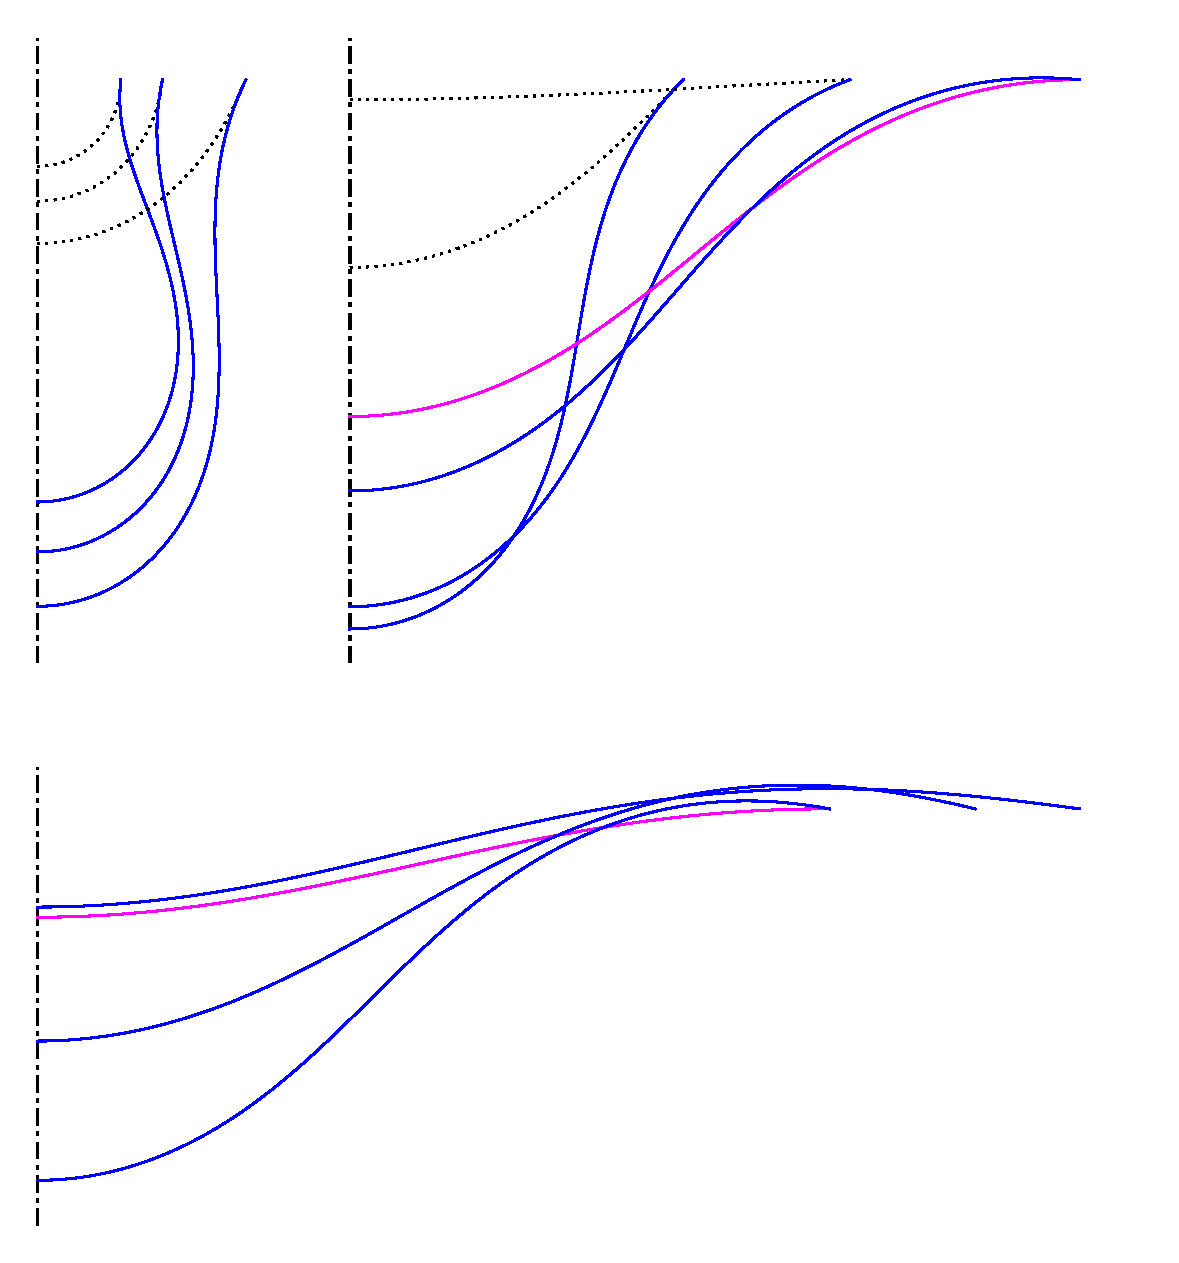
\includegraphics[width=0.6\linewidth]{Pending_Shapes.eps} 
$$
\caption{Pending drops : sample equilibrium shapes for 
$(a)$ $Bo =  0.4, 0.6, 1,$ ; 
$(b)$ $Bo = 1.6, 2.4, 3.6$ ;
$(c)$ $Bo = 3.8, 4.5, 5$. 
The profiles correspond to : maximum pressure (dotted) ; non-axisymmetric instability (grey ; magenta online) ; maximum volume (black ; blue online).
}
\label{fig:PendingShapes}
\end{figure}

\begin{figure}
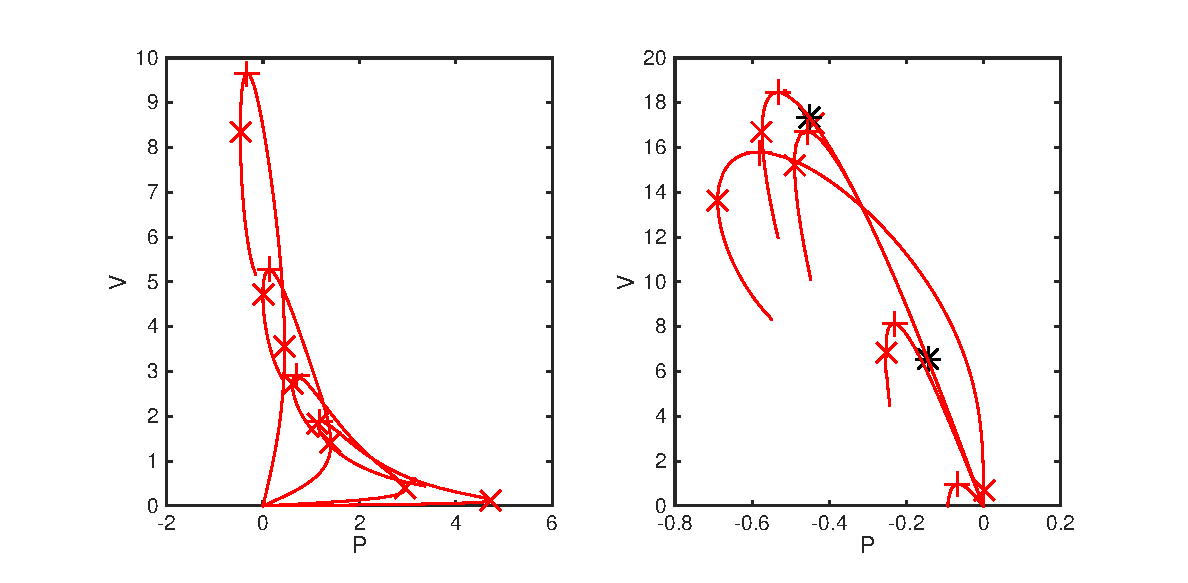
\includegraphics[width=\linewidth]{Pending_PV.eps} 
\caption{Pending drops : V-P curves for  
$(a)$ $Bo = 0.4, 0.6, 1, 1.6$ ; 
$(b)$ $Bo = 2.4, 3.6; 3.8, 4.5, 5$. 
The symbols correspond to : maximum (or minimum) pressure (x) ; maximum volume (+) ;
non-axisymmetric instability (*).
\label{fig:PendingPV}
}
\end{figure}


\begin{figure}
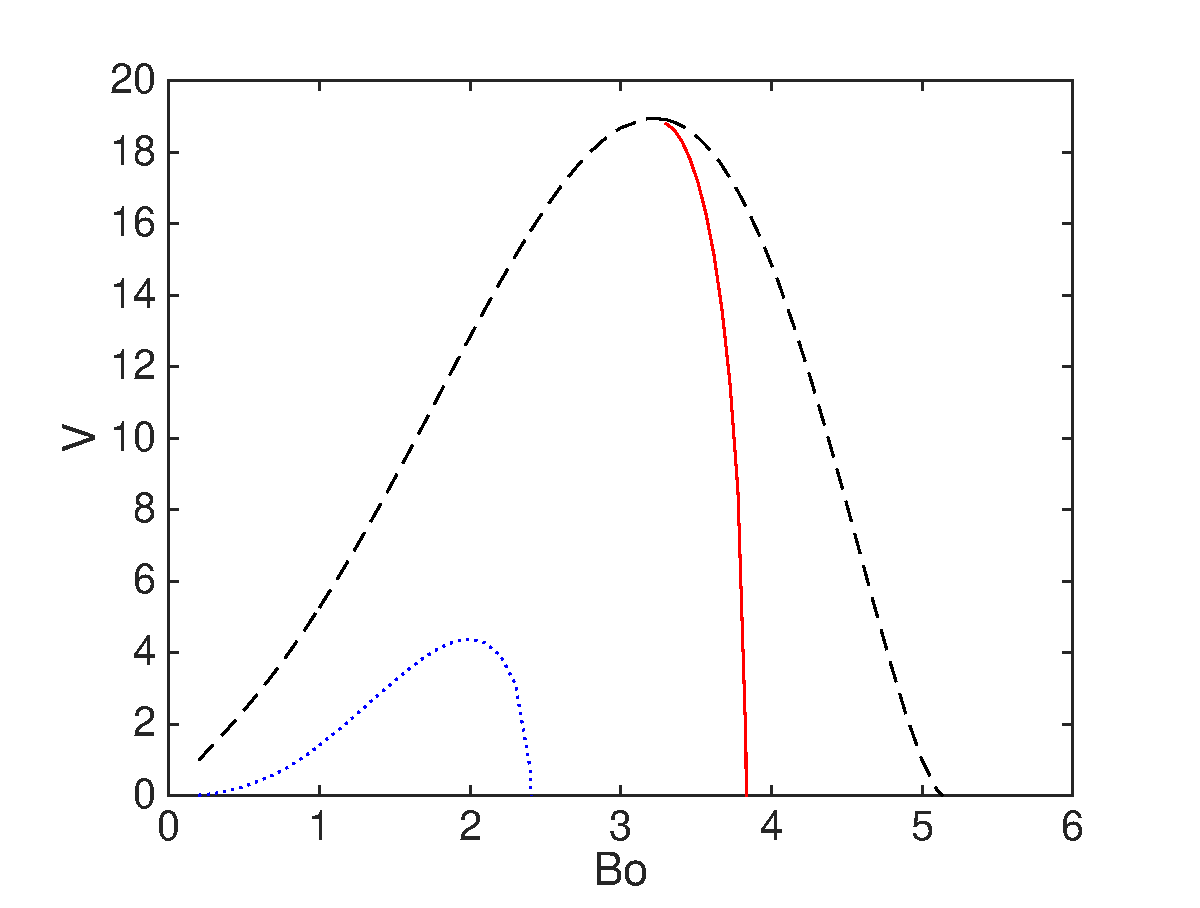
\includegraphics[width=.48\linewidth]{Pending_BoV.eps}
\includegraphics[width=.48\linewidth]{Pending_BoP.eps} 
\caption{
Pending drops : $(a)$ Volume $V$ corresponding to maximum volume (dashed line), 
non-axisymetric stability threshold (plain line), and maximum pressure (dotted line).
$(b)$ Maximum pressure $P$.
}
\label{fig:PendingBoV}
\end{figure}




%\section{Drop pending from a tube (pinned contact line). }
            
            
            
\section{Bubble or drop in oblique gravity}

Assume that gravity is tilted with and angle $\beta$ with respect to the axis $z$ of the nozzle. Assuming $\beta \ll 1$, one can assume that the shape will be displaced by a normal displacement $\beta \eta \cos \theta$ (azimuthal wavenumber $m=1$).

The Young-Taylor equation is :

$$
K_0+ K_1( \beta \eta \cos \theta) = P_0 + \rho g (z_0 + \beta r_0 \cos \theta)
$$

Hence we have to solve :
$$
K_1(\eta) = r_0
$$ 
with boundary conditions $\eta(0) = \eta(s_0) = 0$.


\begin{figure}
$$
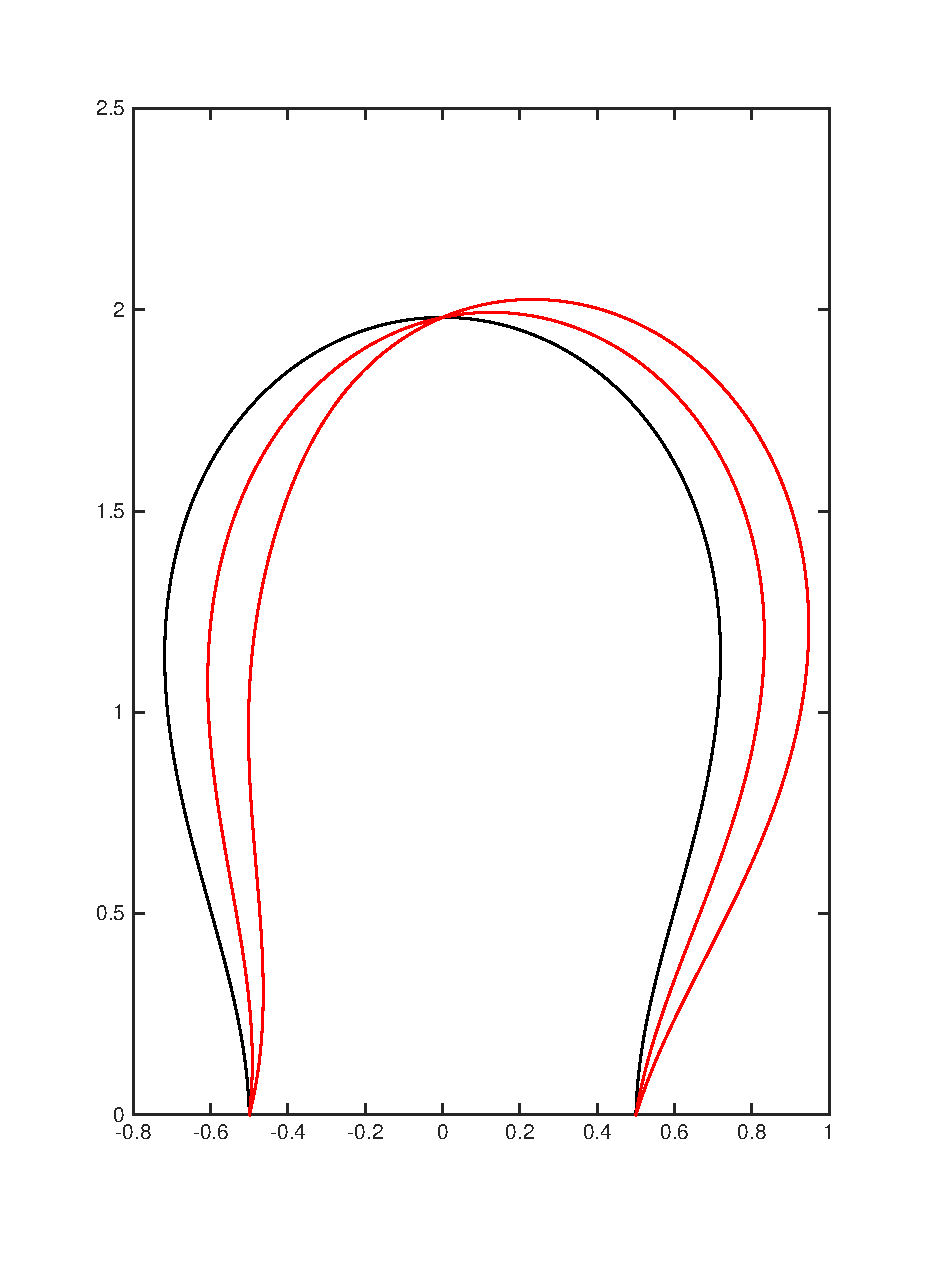
\includegraphics[width=.5\linewidth]{Oblique.eps}
$$
\caption{
Shape of a bubble in oblique gravity, with $Bo = 0.5$, $V = 2.3$, and $\beta = 0.1$ and $0.2$.
}
\end{figure}

The figure shows the result for $Bo = 0.5$, $V = 2.3$, and $\beta = 0.1$ and $0.2$.

The sequence of commands to draw the figure is:
\begin{verbatim}
m = meniscus('flat',100,.5) 
m = m.loop('V',-.1,23)
m = m.oblique(0.1)
m = m.oblique(0.2)
\end{verbatim}
            
            


\section{Conclusion}


\appendix

\section{Numerical implementation in Matlab}

For instance, the data of figure 1 were simply obtained with the following sequence of matlab instructions :

\verb|   m=meniscus('flat',200,2) |

\verb| m = m.loop('S',.01,2000) |

\section{Application to liquid bridges}

\subsection{Weak gravity}

\subsection{Zero gravity}

The equilibrium shapes are computed through an iterative method, described in the appendix (see also Tong Lei Zhang's master). The program is implemented in Matlab language.
The continuation is done with taking as a control parameter either the pressure (=the curvature) inside the bridge (program \verb| Newton_P.m | ), or the volume (program \verb| Newton_V.m |).
The effect of gravity is also implemented.


Once the ratio $L/a$is fixed, the equilibrium shapes form a family which can be parametrized by either the pressure (or curvature), or the volume.

Figure 1 shows the Pressure/Volume relation for three cases ($L/a = 1.3 ; 2 ; 6$),
and figure 2 shows a few shapes in the $R-Z$ plane. Note that starting from the cylindrical bridge, the trend is different for short and long bridges : for short ones increasing the pressure (curvature) leads to an increase of the volume, while for long ones  increasing the pressure (curvature) leads to an decrease of the volume. In all cases, the curve passes through a state of minimum volume, and terminates at a green point where the shape asymptotes to two touching spheres.
We also identify in green the shape which has the same volume as this limit shape. In a coalescence process starting from two touching states, this is the final state, since the volume is conserved during the process and the initial state is unstable.

Note that this final state corresponds corresponds to larger volume than the cylindrical solution for long bridges, and to a smaller volume for short bridges.

The characteristics of these final states are respectively :
For $L/a=1.3$ : $[P,V] = [ -0.01257;  2.3296]$ ; 
For $L/a= 2$ : $[P,V] = [ 0.7428 ;  4.1888 ]$ ; 
For $L/a = 4$ : $[P,V] = [  0.9699 ; 14.6607]$ ;
For $L/a= 6$ : $[P,V] = [0.7926 ; 37.7]$.

Note also that in the case $L/a = 1.3$, the problem admits two solutions with zero pressure (or curvature), which correspond to classical catenoidal shapes. These cases are identified in blue.
 




\begin{figure}
\begin{tabular}{cc}
\includegraphics[width=.45\linewidth]{PV_Bridge_L1_3.pdf} &
\includegraphics[width=.45\linewidth]{PV_Bridge_L2.pdf} \\
$(a)$ : $L/a = 1.3$ & $(b)$ : $L/a = 2$ \\
\includegraphics[width=.45\linewidth]{PV_Bridge_L4.pdf} & 
\includegraphics[width=.45\linewidth]{PV_Bridge_L8.pdf} \\
$(c)$ : $L/a = 4$ & $(d)$ : $L/a = 6$ \\
\end{tabular}
\caption{Pressure-volume relations for equilibrium shapes, for $L/a= 1.3; 2; 4$ and $6$. Circles identify the cylindrical shape (red), the limit shape of touching spheres (green), the shape with same volume (green), and (for $L/a= 1.3$) the catenoidal shapes (blue). }
\end{figure}

\begin{figure}
$$
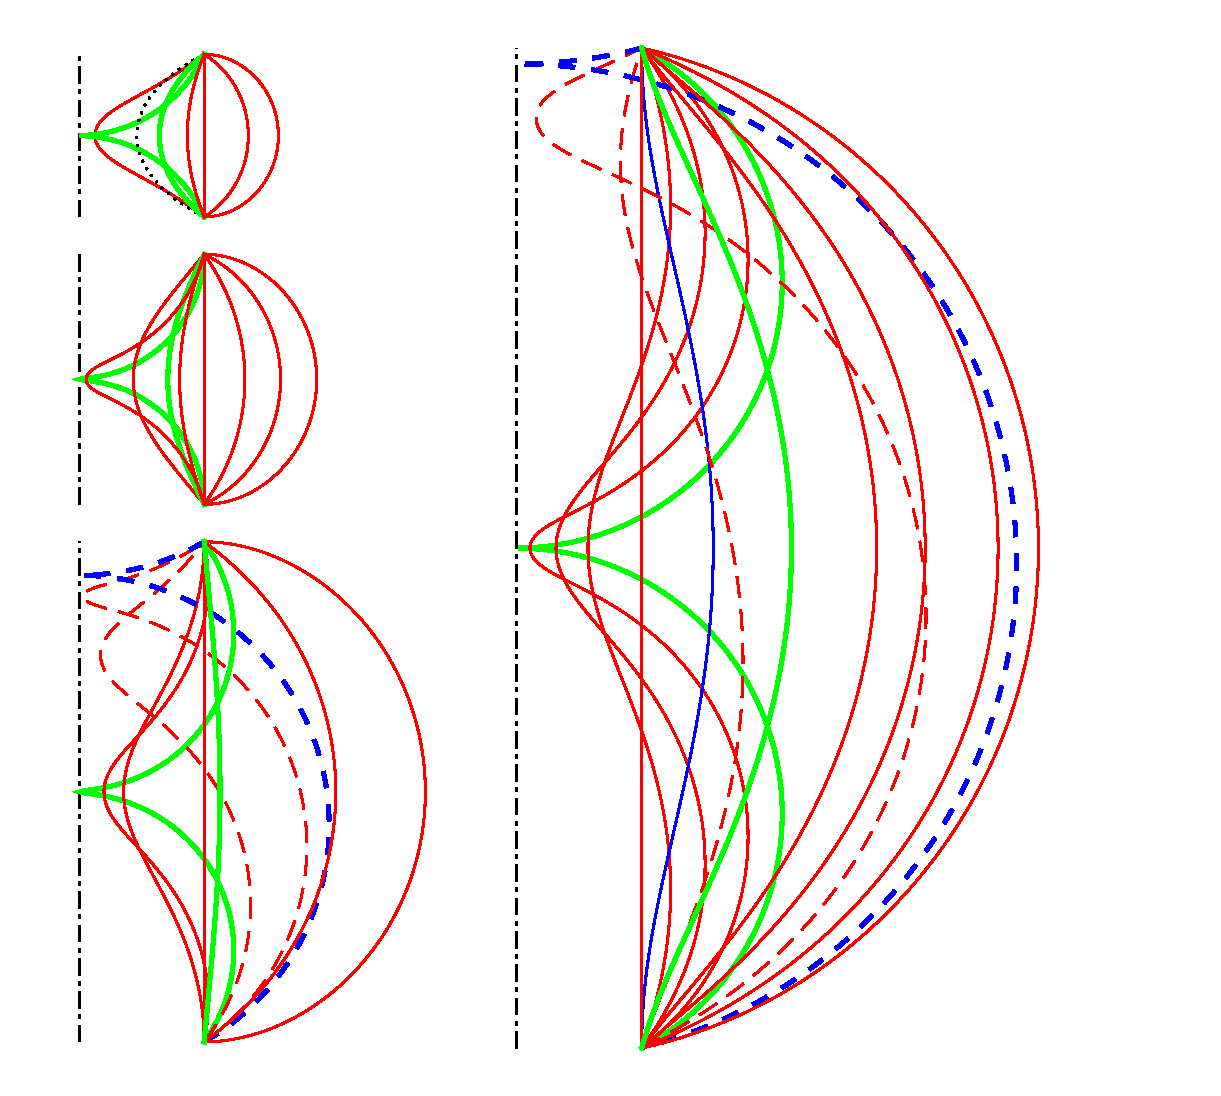
\includegraphics[width=.8\linewidth]{Bridges_Shapes.eps}
$$
\caption{Sample equilibrium shapes of liquid bridges with zero gravity, 
for $(a)$ $L/a= 1.3$, $(b)$ $L/a=2$, $(c)$ $L/a=4$, and $(d)$ $L/a=8$.
In all cases, the thick, grey (green online) contours correspond to the limit case of two touching spheres of equal size and to the shape with same volume ; in $(a)$ the dotted line corresponds to  a catenoid shape;
in $(c)$ and $(d)$ the dashed contours are asymmetric shapes and the thick, dashed one is the limit case of two touching spheres of unequal size. }
\end{figure}


     



%\subsection{Drop pending from a ceiling (angle-controlled contact line).}




\end{document}




\section{Liquid bridges (no gravity)}
            
%\begin{abstract}
%\end{abstract}
%\begin{keywords}
%\end{keywords}


\clearpage

\appendix

%\end{document} 
 

\section{Appendix}



\subsection{Cas particulier : forme moyenne sphérique}

On suppose que la forme moyenne est une sphère de rayon $R_0$. On utilise les coordonnées sphériques $(R,\Theta)$. Dans ce cas, l'abscisse curviligne de la forme moyenne $s_0$ est donné par 
$s_0  = R_0 \Theta$, et on a :
$$
r = R_0 \sin \Theta ; \quad z = R_0 \cos \Theta; \quad \DP{}{s_0} = \frac{1}{R_0} \DP{}{\Theta}
$$
$$
{\bf N_0} = {\bf e_R} ; \quad {\bf T_0} = {\bf e_\Theta} ; \quad N_{0,r} = \sin \Theta; 
$$

En injectant dans les formules précédentes, on aboutit à :
$$
K_0 = \frac{2}{R_0}
$$
$$ 
K_1 = - \frac{1}{R_0^2 \sin \Theta} \DP{}{\Theta} \left( \sin \Theta \DP{\eta}{\theta} \right) 
- \frac{2}{R_0^2} \eta
$$
Ce qui correspond bien aux formules obtenues dans ce cas.

\subsection{Paramétrage selon $r$}

Vérifions que les formules générales trouvée ici est équivalente à celles utilisées dans le cas où la surface est paramétrée par $r$ et non par $s_0$ C'est-à-dire : 

$$
z = H(r) = h_0(r) + \epsilon \eta_z (r)
$$

Dans ce cas le calcul de la courbure conduit à :
$$
K =  K_0(r) + \epsilon k(r)
$$

avec :
$$
K_0(r) = -\frac{1}{r} \DP{}{r} \left( \frac{r}{\sqrt{1+ h_0'^2}} \DP{h_0}{r} \right)
$$

$$
k(r) = -\frac{1}{r} \DP{}{r} \left( \frac{r}{\left(1+ h_0'^2\right)^3} \DP{\eta_z}{r} \right) 
$$

(Par rapport aux formules données dans le rapport de Jérôme on a changé les signes afin d'utiliser la même convention sur les normales, et on a rectifié une petite erreur dans le terme $k$).


La correspondance entre les deux formulations s'établit en utilisant les identités suivantes :

$$ 
\eta_z(r) = \frac{\eta(s_0)}{N_{0,z}}  ; 
\quad 
T_{0,r} = N_{0,z} = \frac{1}{\sqrt{1+ h_0'^2}}; 
\quad 
T_{0,z} = -N_{0,r} =  \frac{h_0'}{\sqrt{1+ h_0'^2}}
$$

$$
\DP{}{r} = N_{0,z} \DP{}{s_0}
$$

$$
k(r) = K_1(s_0)  - \DP{K_0}{s_0} T_{0,z} \eta_z(r)
$$

(formules vérifiées avec Maple)



\subsection{Implémentation avec Freefem}

Pour le calcul de la courbure moyenne, il faut commencer par interpoler les vecteurs normal (et tangent) 
sous forme de champs P1 définis sur la frontière :



\begin{verbatim}
(...)

mesh Shempty=emptymesh(Sh);
fespace Wh1(Shempty,P1);
Wh1 N0r,N0z,T0r,T0z,K0a,K0b,test ;

problem CalcN0r(N0r,test)=
 int1d(Shempty,qfe=qf3pE)(N0r*test)-int1d(Shempty,qfe=qf3pE)(N.x*test);
problem CalcN0z(N0z,test)=
 int1d(Shempty,qfe=qf3pE)(N0z*test)-int1d(Shempty,qfe=qf3pE)(N.y*test);

CalcN0r;
CalcN0z;
T0r =  N0z;
T0z = -N0r;

macro Ds(u1,u2)
[dx(u1)*T0r+dy(u1)*T0z,dx(u2)*T0r+dy(u2)*T0z]
//

problem ComputeK0a(K0a,test)=
 int1d(Shempty,qfe=qf3pE)(K0a*test)
-int1d(Shempty,qfe=qf3pE)(Ds(N0r,N0z)'*[T0r,T0z]*test);
ComputeK0a;

problem ComputeK0b(K0b,test)=
 int1d(Shempty,qfe=qf3pE)(K0b*test*x)
-int1d(Shempty,qfe=qf3pE)(N0r*test);
ComputeK0b;


\end{verbatim}


Pour les perturbations, le terme de courbure se traite par intégration par partie :

$$
p = \sigma K_1 
$$
$$
\int_{\cal S}  \eta^\dag p r d \ell 
 = \sigma 
 \int_{\cal S} \left (
 \DP{\eta^\dag}{s_0} \DP{\eta}{s_0} - \left[ \left| \DP{\bf N_0}{s_0} \right|^2  + \frac{N_{0,r}^2}{r^2} \right]  \eta^\dag \eta \right) r d \ell 
\mbox{ (+ termes de bord)} 
$$




\section{Spilling drops}


\begin{figure}
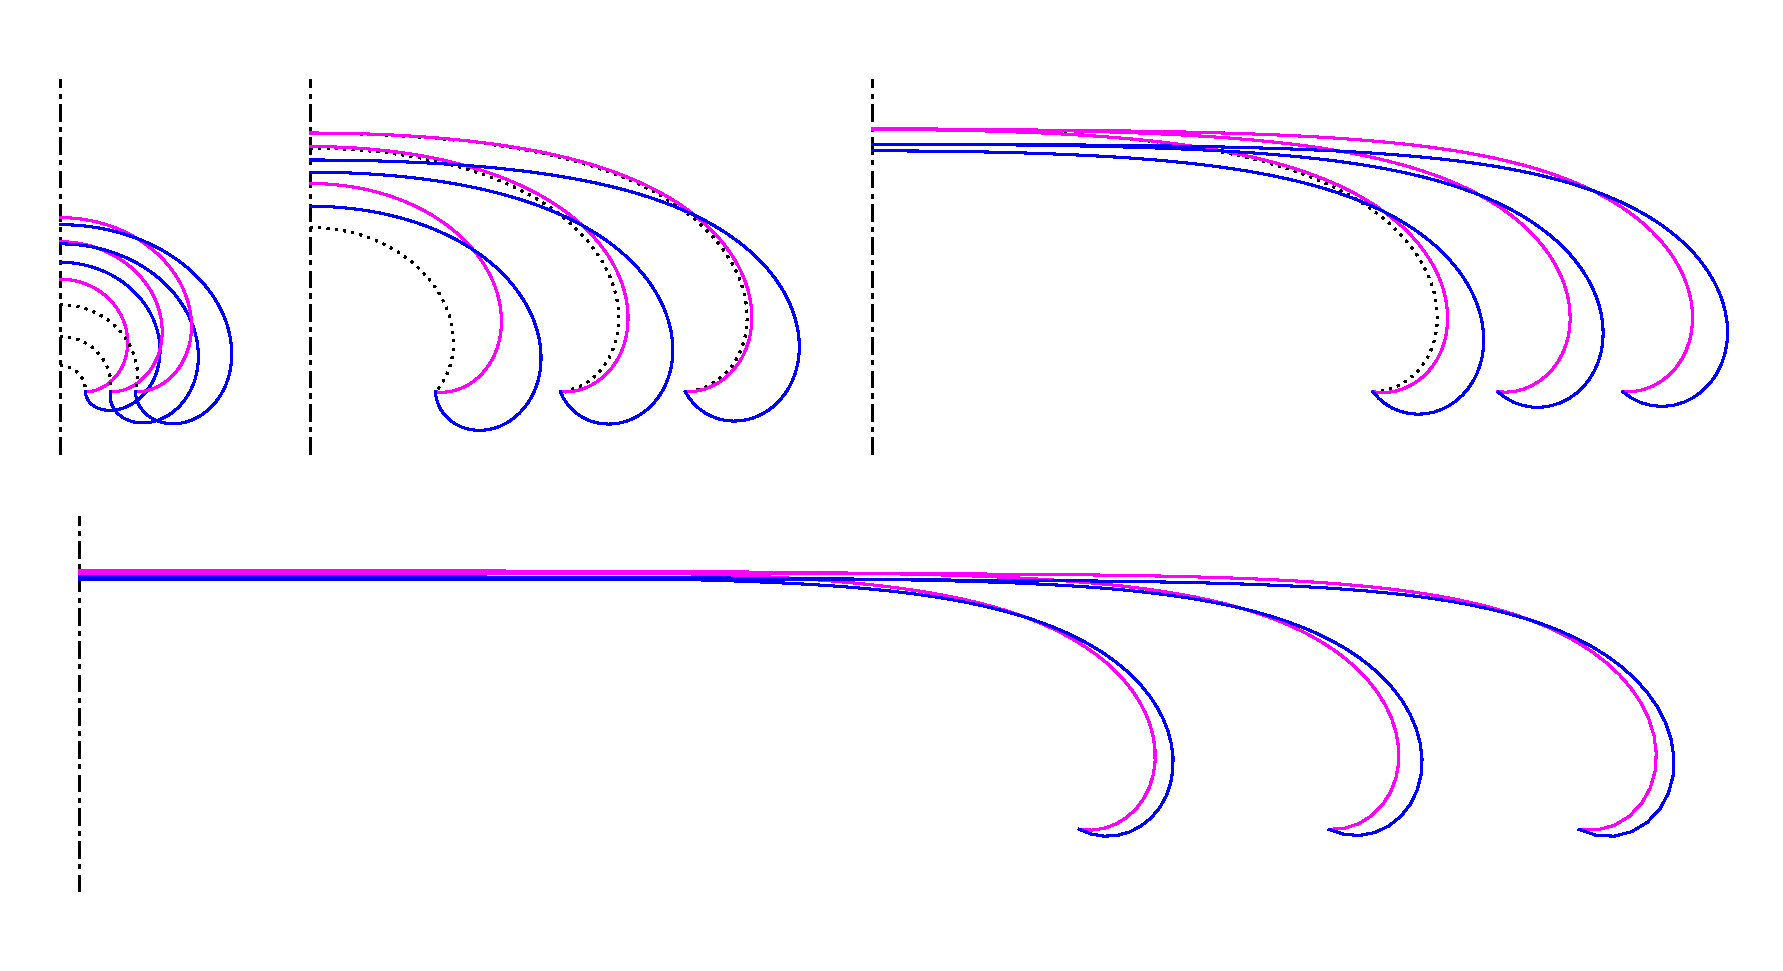
\includegraphics[width=\linewidth]{Sessile_Shapes.eps} 
\caption{Spilling drops : sample equilibrium shapes for 
$(a)$ $Bo = 0.2, 0.4, 0.6$ ; 
$(b)$ $Bo = 1, 2, 3$ ;
$(c)$ $Bo = 4, 5, 6$ ;
$(d)$ $Bo = 8, 10, 12$. 
In each case the three profiles correspond to : maximum pressure (magenta) ; non-axisymmetric instability (green) ; maximum volume (blue).
}
\end{figure}

\begin{figure}
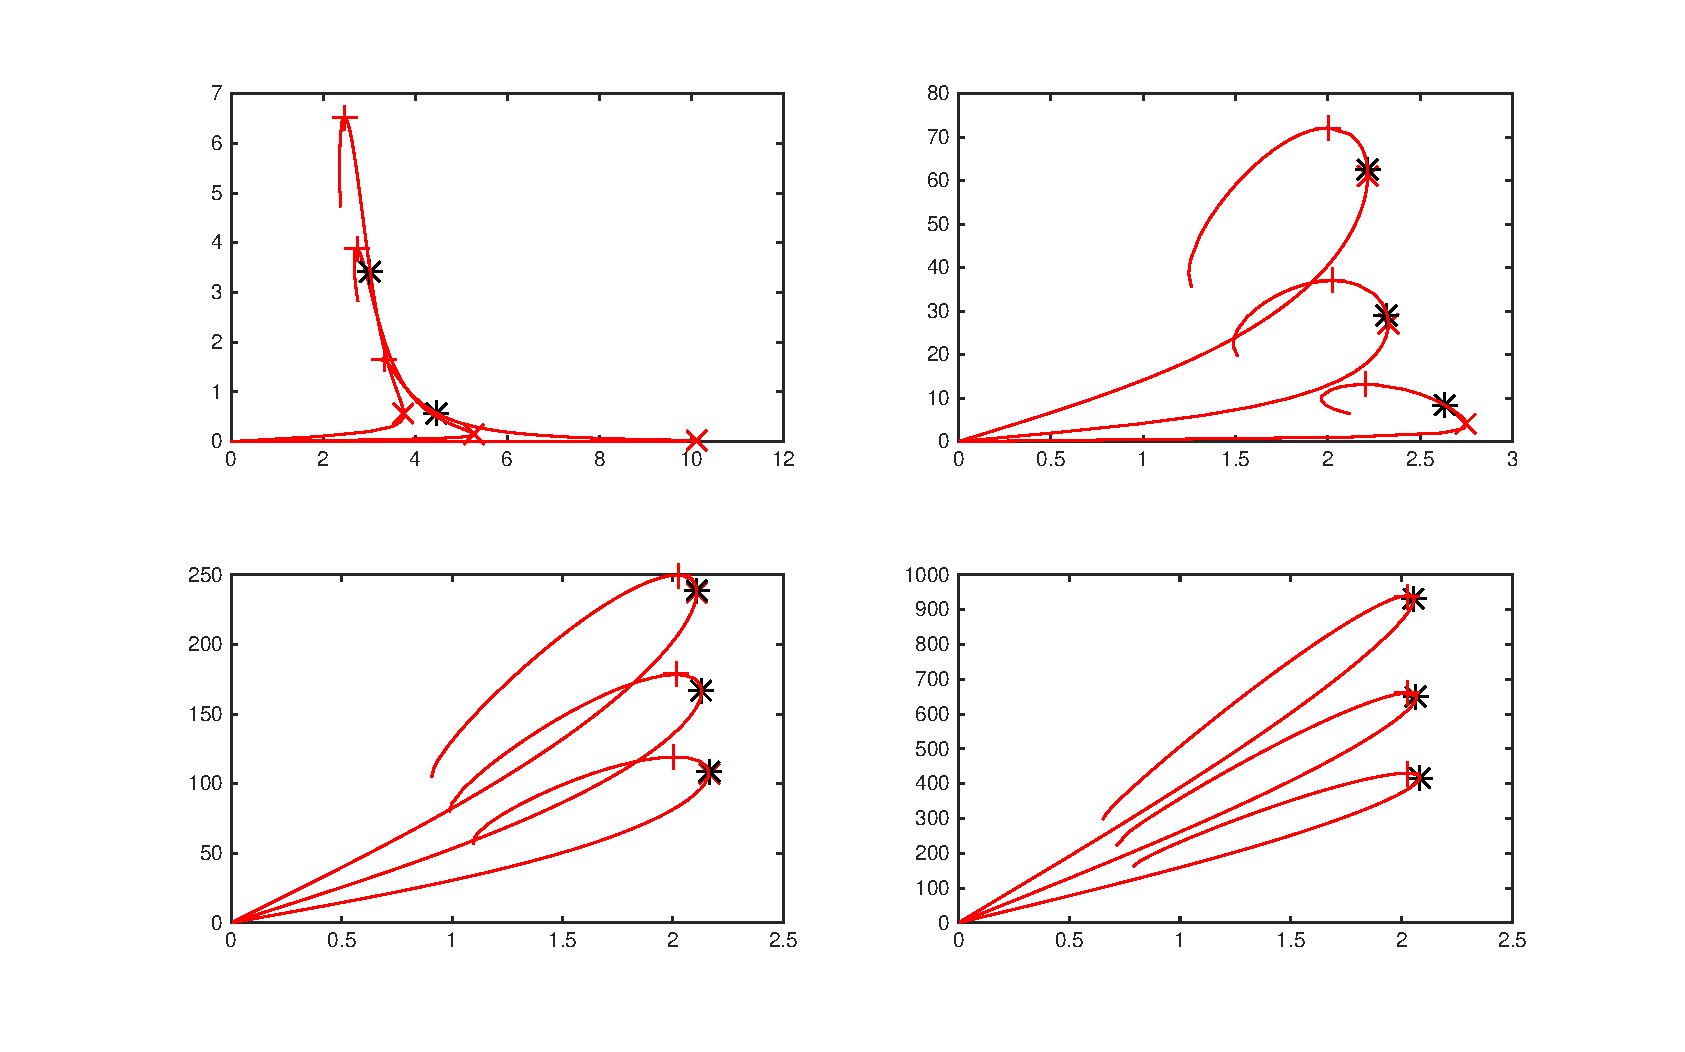
\includegraphics[width=\linewidth]{Sessile_PV.eps} 
\caption{Spilling drops : V-P curves for  
$(a)$ $Bo = 0.2, 0.4, 0.6$ ; 
$(b)$ $Bo = 1, 2, 3$ ;
$(c)$ $Bo = 4, 5, 6$ ;
$(d)$ $Bo = 8, 10, 12$. 
The symbols correspond to : maximum pressure (x) ; non-axisymmetric instability (*) ; maximum volume (+).
}
\end{figure}


\begin{figure}
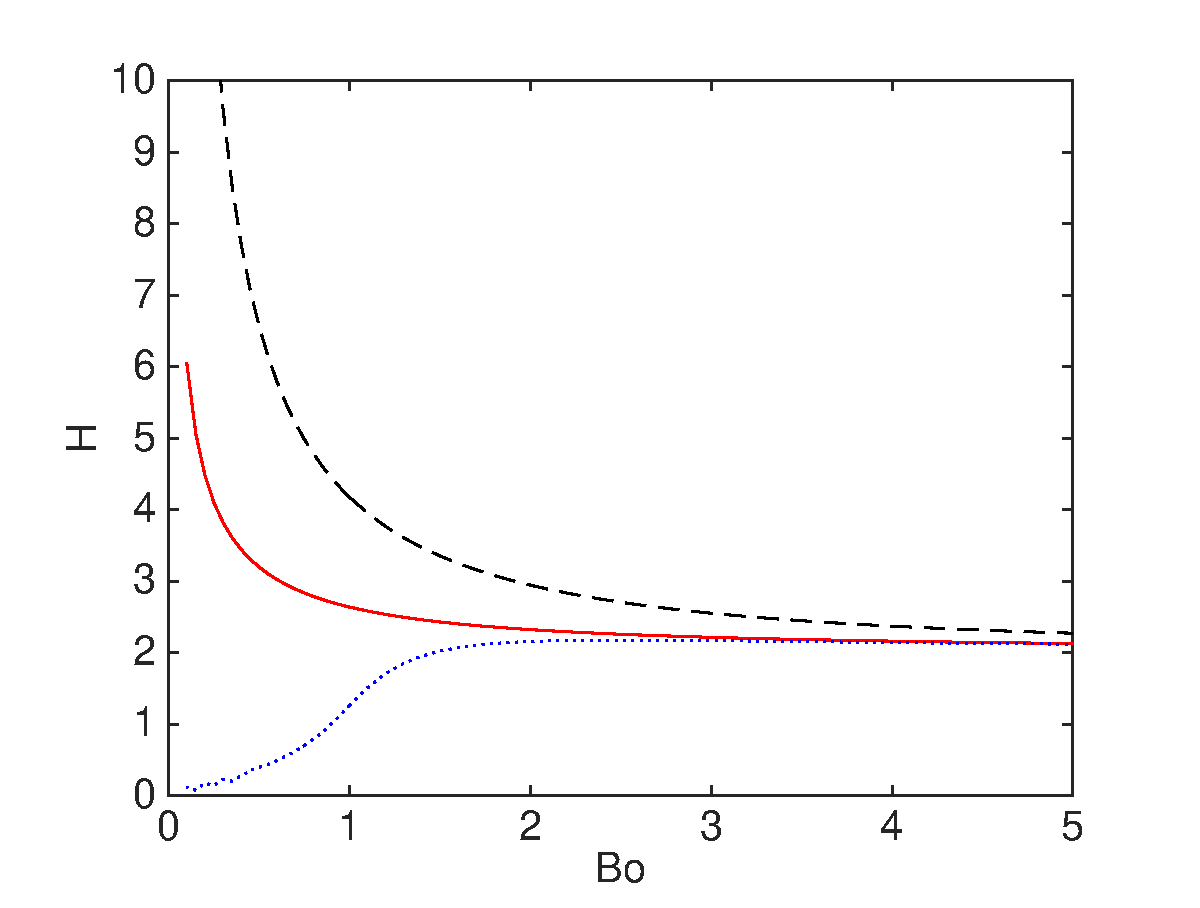
\includegraphics[width=.48\linewidth]{Sessile_BoV.eps}
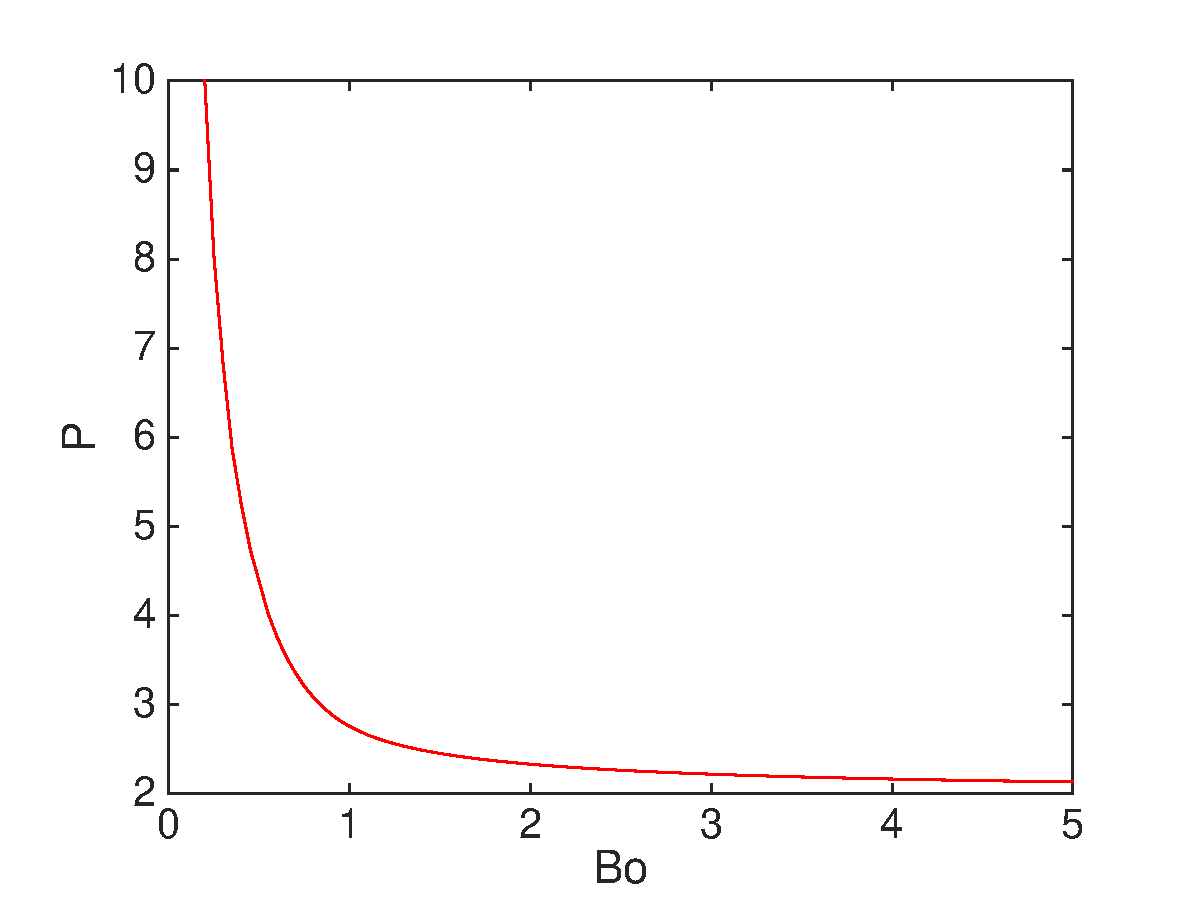
\includegraphics[width=.48\linewidth]{Sessile_BoP.eps} 
\caption{
Spilling drops : $(a)$ Equivalent height $H = V/(\pi Bo^2)$ corresponding to non-axisymetric stability threshold (plain line), maximum volume (dashed line), and maximum pressure (dotted line).
$(b)$ Maximum pressure $P$.
}
\end{figure}




%%%%%%%%%%%%%%%%%%%%%%%%%%%%%%%%%

\end{document}


\begin{figure}
\vcenteredhbox{
\begin{tabular}{c}
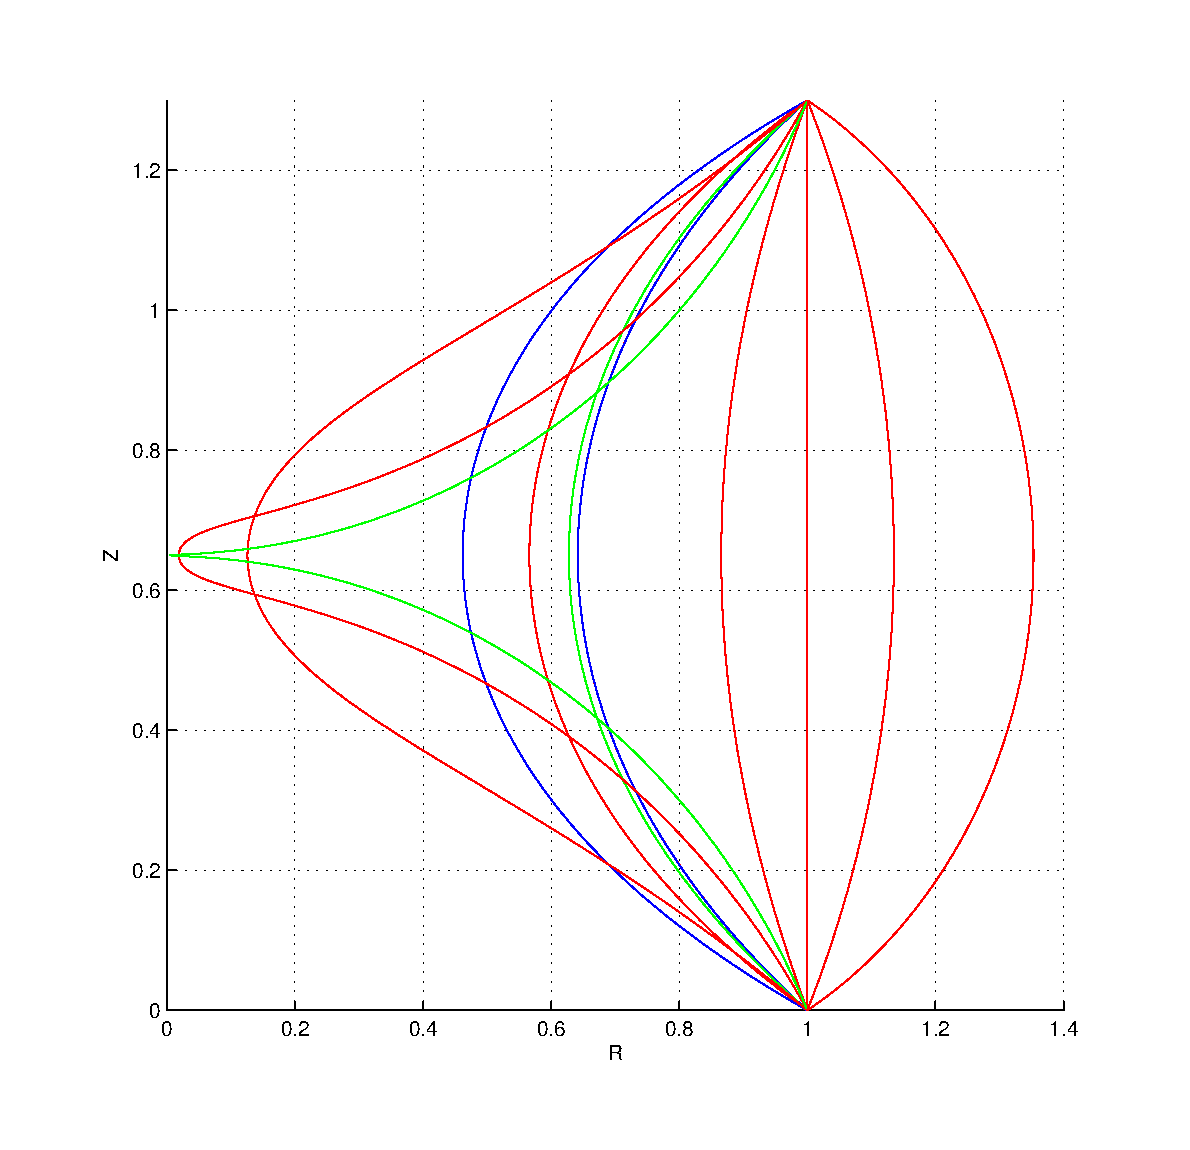
\includegraphics[width=.4\linewidth]{ShapeBridges_L1_3.eps}
\\
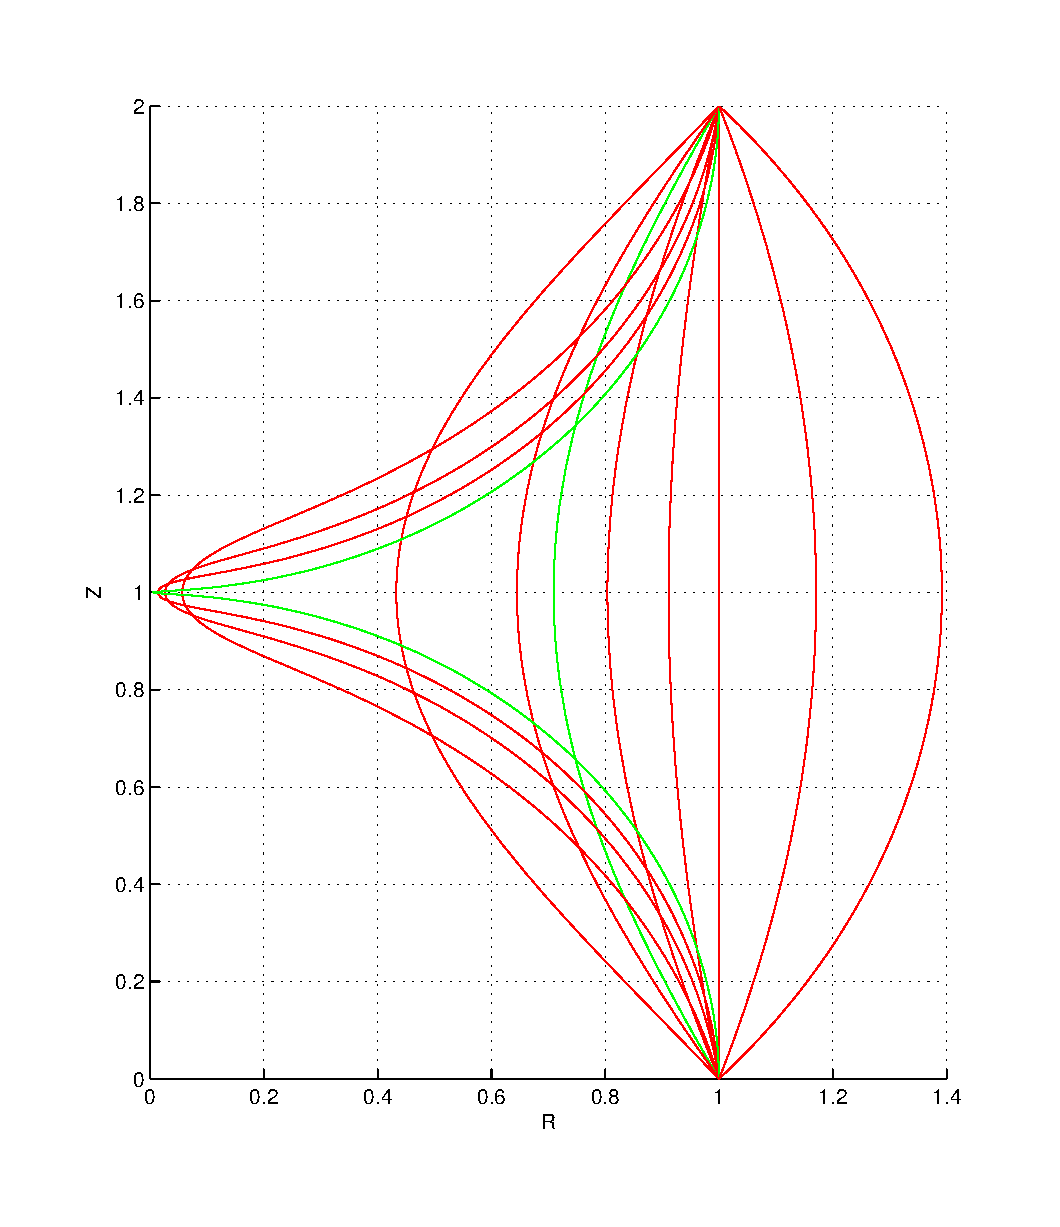
\includegraphics[width=.4\linewidth]{ShapeBridges_L2.eps}
\end{tabular}
}
\vcenteredhbox{
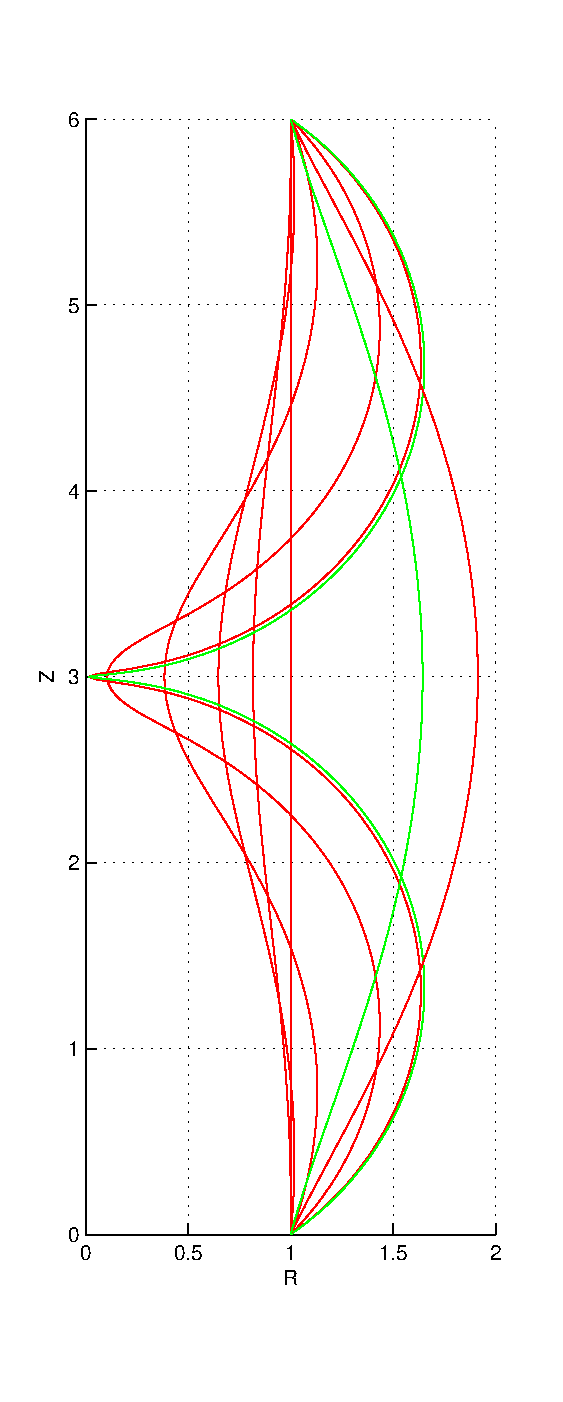
\includegraphics[width=.4\linewidth]{ShapeBridges_L6.eps}
}
\caption{A few equilibrium shapes for liquid bridges, for $L/a= 1.3$, $2$ and $6$.
The green shapes correspond to the limit case where the bridge becomes two touching spherical portions, and to the configuration with the same volume. }
\end{figure}




